\documentclass{beamer}



\usetheme{Madrid}

\usepackage[utf8]{inputenc}
\usepackage[russian]{babel}
\usepackage{hyperref}
\usepackage[noline, noend, onelanguage, boxed]{algorithm2e}


\SetKwInput{KwData}{Исходные параметры}
\SetKwInput{KwResult}{Результат}
\SetKwInput{KwIn}{Вход}
\SetKwInput{KwOut}{Выход}
\SetKwIF{If}{ElseIf}{Else}{если}{тогда}{иначе если}{иначе}{конец условия}
\SetKwFor{While}{до тех пор, пока}{выполнять}{конец цикла}
\SetKw{KwTo}{от}
\SetKw{KwRet}{вернуть}
\SetKw{Return}{вернуть}
\SetKwBlock{Begin}{начало}{конец}
\SetKwSwitch{Switch}{Case}{Other}{Проверить значение}{и выполнить}{вариант}{в противном случае}{конец варианта}{конец проверки значений}
\SetKwFor{For}{для}{:}{конец цикла}
\SetKwFor{ForEach}{для каждого}{выполнять}{конец цикла}
\SetKwFor{ForAll}{для всех}{выполнять}{конец цикла}
\SetKwRepeat{Repeat}{повторять}{до тех пор, пока}
\SetAlgorithmName{Алгоритм}{алгоритм}{Список алгоритмов}

\title[]{Задача поиска графа-паттерна на помеченном графе}
\author[Мурадьян И.В.]{Мурадьян Илья Валерьевич}
\institute[ЮФУ ИММиКН]{Прикладная математика и информатика \\
	Кафедра алгебры и дискретной математики \\
	Научный руководитель: доцент, д.ф.-м.н Скороходов Владимир Александрович \\
}
\date{Июнь 2018}
 
\begin{document}
 
\frame{\titlepage}
 
\begin{frame}
\frametitle{Цели и задачи работы}
\begin{enumerate}
	\item Провести исследование задачи поиска графа-паттерна на помеченном графе в случае, когда метки вершин являются уникальными.
	\item Провести исследование задачи поиска графа-паттерна на помеченном графе в случае, когда метки вершин \textbf{не} являются уникальными.
	\item Разработать алгоритмы:
	\begin{itemize}
		\item исключения вершин по локальным условиям;
		\item проверки контуров возможных совпадений;
		\item выделения взвешенного совпадения подграфов.
	\end{itemize}
\end{enumerate}
\end{frame}
 
\begin{frame}
\frametitle{Задача поиска графа-паттерна на помеченном графе}
 \textbf{Задача}: найти частичный подграф архивного графа $G$, изоморфный графу-паттерну $G'$.
 \begin{figure}[H]
 	\centering
 	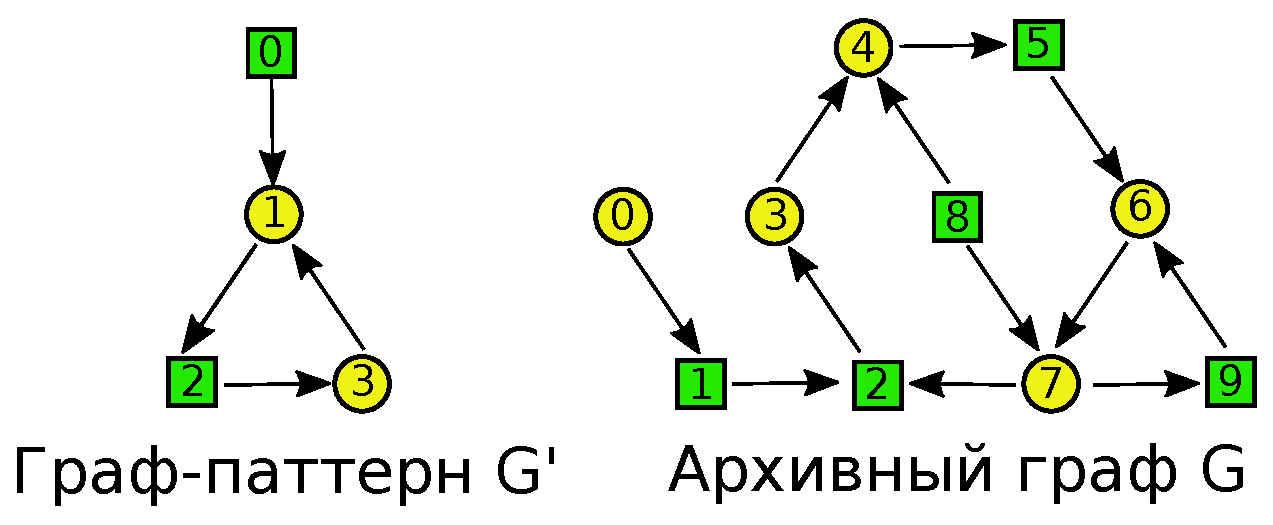
\includegraphics[width=1\textwidth]{ee}
 	\label{fig:ee}
 \end{figure}
\end{frame}

\begin{frame}
\frametitle{Возможные практические приложения}
\begin{enumerate}
	\item Поиск симметричных графов-паттернов при обработке изображений.
	\item Поиск иерархических структур в графах социальных взаимодействий.
\end{enumerate}
\begin{figure}[H]
	\centering
	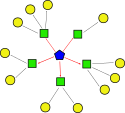
\includegraphics[width=0.5\textwidth]{ierar}
	\label{fig:ierar}
\end{figure}
\end{frame}

\begin{frame}
\frametitle{Общий алгоритм исключения кандидатов}

Отображение кандидатов $f : V' \to 2^V$ сопоставляет вершинам графа-паттерна возможно соответствующие им вершины архивного графа.

\begin{algorithm}[H]
	\KwIn{графы $G(V, E)$, $G'(V', E')$}
	\Begin(Exclusion){		
		Инициализировать отображение кандидатов $f$
		
		\While{вершины продолжают исключаться}{
			$f := LocalConstraintsChecking(G, G', f, N)$
			
			$f := CycleChecking(G, G', f)$
		}
		\Return{$f$}
	}
\end{algorithm}

Алгоритм заключается в исключении как можно большего числа несоответствующих вершин из множеств $f(v')$.

\end{frame}

\begin{frame}
\frametitle{Пример: инициализация}
\begin{figure}[H]
	\centering
	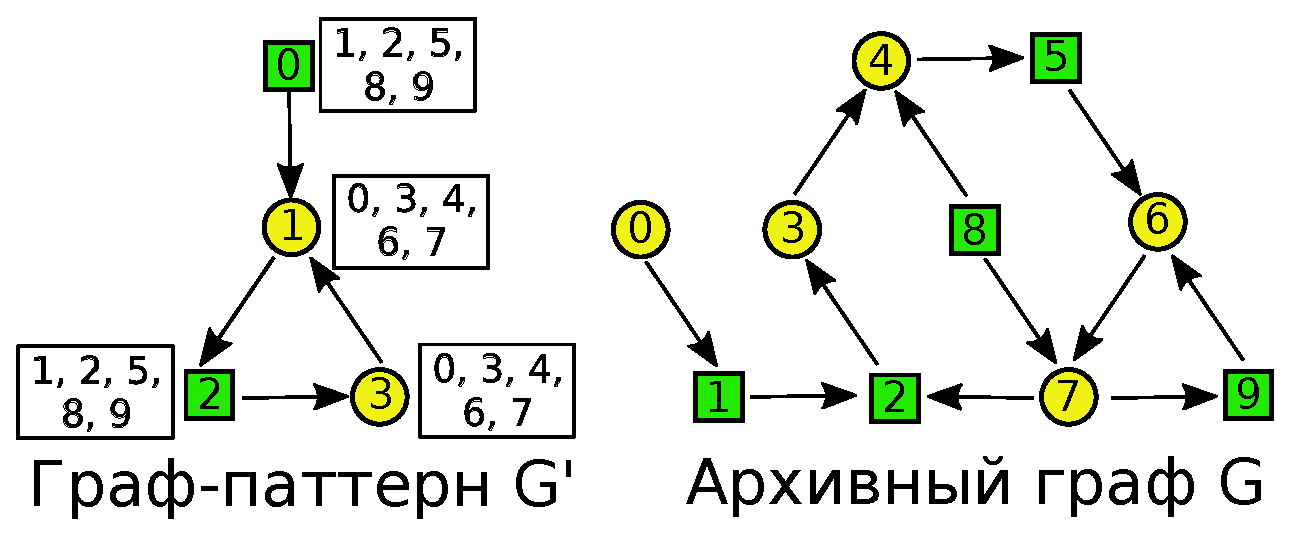
\includegraphics[width=1\textwidth]{ee9}
	\label{fig:ee9}
\end{figure}
\end{frame}

\begin{frame}
\frametitle{Алгоритм исключения по локальным условиям}
\begin{algorithm}[H]
	\KwIn{$G(V, E)$, $G'(V', E')$, $f$, число итераций $N$}
	\Begin(LocalConstraintsChecking){		
		\For{$i = 1, 2, .., N$}{
			\For{$(q_0, q) \in E'$}
			{
				\For{$v_0 \in f(q_0)$}{
					$flag := False$
					
					\For{$v \in \Gamma(v_0)$}{
						\If{$v \in f_K(q)$ и $\rho(\chi(v_0, v), \chi'(q_0, q)) = 1$}{
							$flag := True$
						}
					}
					
					\If{$flag = False$}{
						Исключить $q_0$ из $f(v_0)$
					}
				}
				
				Аналогично -- для обратных дуг
			}
		}
		\Return{$f$}
	}
\end{algorithm}

Сложность на одной итерации: $O(|E'|\cdot|V|^2)$.
\end{frame}

\begin{frame}
\frametitle{Пример: шаг 1, алгоритм исключения по локальным условиям}
\begin{figure}[H]
	\centering
	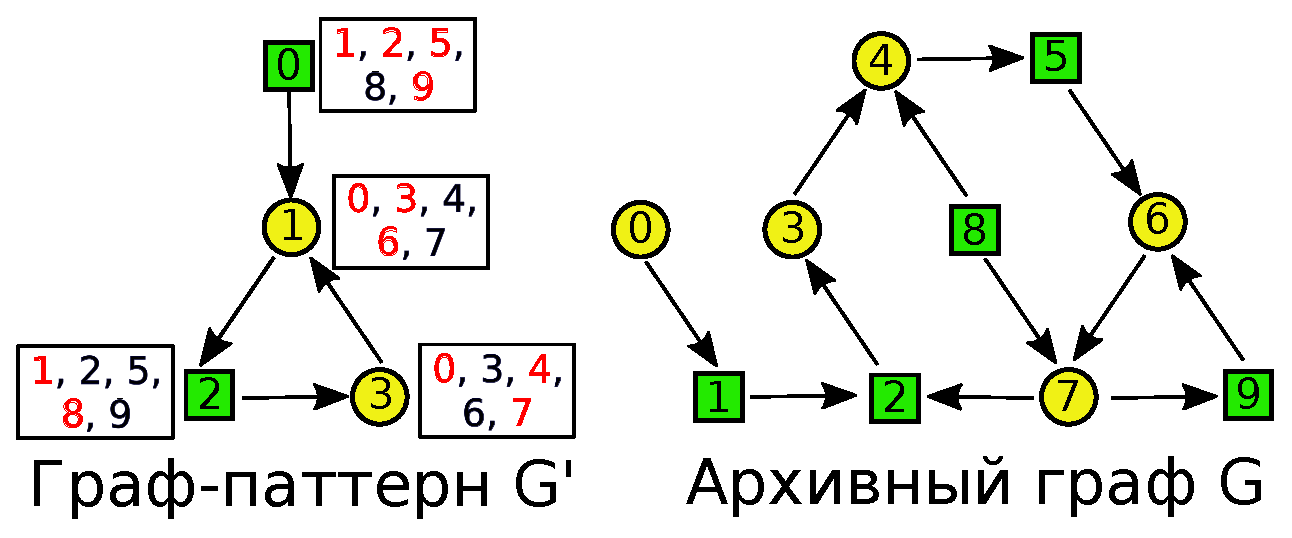
\includegraphics[width=1\textwidth]{ee1}
	\label{fig:ee1}
\end{figure}
\end{frame}

\begin{frame}
\frametitle{Алгоритм проверки контуров}
$\mathcal{K}_0$ -- множество проверяемых контуров.

\begin{algorithm}[H]
	\KwIn{$G(V, E)$, $G'(V', E')$, $f$}
	\Begin(CycleChecking){
		\ForEach{$\mathcal{C}_0 \in \mathcal{K}_0$}{
			Пусть $(v_0^{\prime}, v_1^{\prime})$ -- первая дуга контура $\mathcal{C}_0$.
			
			Исключить из множества $f(v_0^{\prime})$ те вершины, в которых не начинается контур, соответствующий $\mathcal{C}_0$.
		}
		\Return{$f$}
	}
\end{algorithm}

Сложность: $O(|\mathcal{K}_0| \cdot |V|^3 \cdot |E'|)$.
\end{frame}

\begin{frame}
\frametitle{Пример: шаг 1, алгоритм проверки контуров}
\begin{figure}[H]
	\centering
	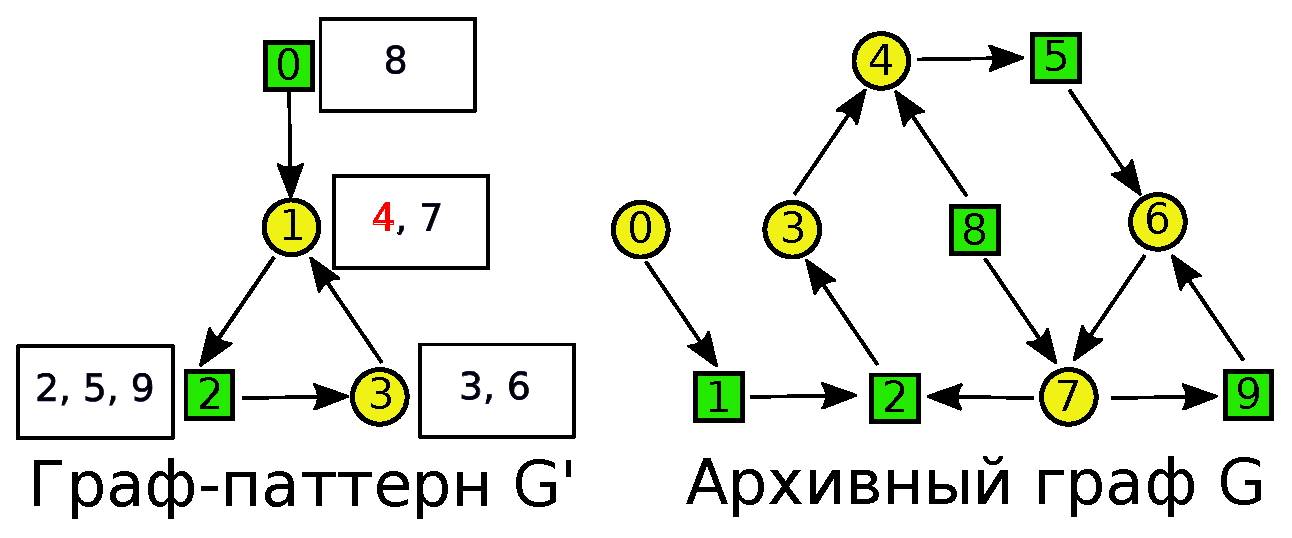
\includegraphics[width=1\textwidth]{ee4}
	\label{fig:ee4}
\end{figure}
\end{frame}

\begin{frame}
\frametitle{Пример: шаг 2, алгоритм исключения по локальным условиям}
\begin{figure}[H]
	\centering
	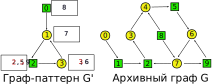
\includegraphics[width=1\textwidth]{ee5}
	\label{fig:ee5}
\end{figure}
\end{frame}

\begin{frame}
\frametitle{Пример: окончательный результат}
\begin{figure}[H]
	\centering
	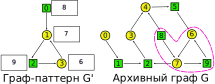
\includegraphics[width=1\textwidth]{ee7}
	\label{fig:ee7}
\end{figure}
\end{frame}

\begin{frame}
\frametitle{Возможные проблемы}
Применение общего алгоритма не гарантирует исключения всех кандидатов. В частности, в нижеприведённом случае не происходит исключения несоответствующих вершин.

\begin{figure}[H]
	\centering
	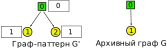
\includegraphics[width=1\textwidth]{problem}
	\label{fig:problem}
\end{figure}

Решения: проверить степени вершин при инициализации, применить алгоритм выделения взвешенного совпадения в конце.
\end{frame}

\begin{frame}
\frametitle{Алгоритм выделения взвешенного совпадения}
\begin{enumerate}
	\item Преобразовать граф-паттерн $G'$ к особому виду, снабдив его дополнительной информацией, получив таким образом граф $G_0$.
	\item Положить $i := 0$.
	\item Пока граф $G_i$ имеет более одной вершины:
	\begin{enumerate}
		\item Выполнить на графе $G_i$ обход в ширину с окраской.
		\item Выделить подграфы графа $G_i$ с вершинами одного цвета.
		\item На каждом выделенном подграфе $G_i^j(V_i^j, E_i^j)$ построить все возможные соответствия между его вершинами и вершинами архивного графа.
		\item Сформировать новый граф $G_{i+1}$, взяв в качестве вершин подграфы $G_i^j$, а в качестве дуг -- дуги, вершины которых принадлежат сразу нескольким подграфам.
		\item Положить $i := i + 1$.
	\end{enumerate}
\end{enumerate}
\end{frame}

\begin{frame}
\frametitle{Полученные результаты}
\begin{enumerate}
	\item Проведено исследование задачи поиска графа-паттерна на помеченном графе в случаях, когда метки на графе-паттерне уникальны и когда они неуникальны.
	\item Рассмотрена возможность нахождения графов-паттернов не только по вершинам, но и по дугам.
	\item Разработаны алгоритмы, требуемые по заданию.
	\item Разработанные алгоритмы реализованы, репозиторий: \url{https://github.com/ileasile/diploma/tree/master/python_graph_pattern_project}
\end{enumerate}
\end{frame}
 
\end{document}